\documentclass{standalone}
\usepackage{tikz}

\begin{document}

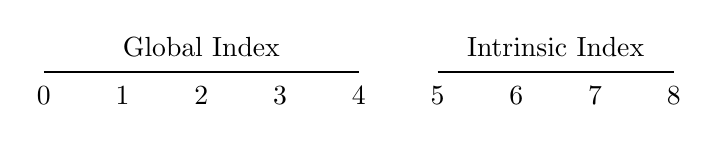
\begin{tikzpicture}
  % Draw the first segment (Global Index) from 0 to 4
  \draw[thick] (0,0) -- (4,0) node[midway, above=2pt] {Global Index};
  % Draw the second segment (Intrinsic Index) from 5 to 8 (with a gap after 4)
  \draw[thick] (5,0) -- (8,0) node[midway, above=2pt] {Intrinsic Index};
  % Add numerical markers along the line (below the line)
  \node at (0,-0.3) {0};
  \node at (1,-0.3) {1};
  \node at (2,-0.3) {2};
  \node at (3,-0.3) {3};
  \node at (4,-0.3) {4};
  \node at (5,-0.3) {5};
  \node at (6,-0.3) {6};
  \node at (7,-0.3) {7};
  \node at (8,-0.3) {8};
\end{tikzpicture}

\end{document}